%!TeX root=../main.tex

In biology, precocial species are those whose young already possess certain abilities from the moment of birth. There is evidence to show that lizard~\cite{miles1995morphological} and snake~\cite{burger1998antipredator,mori2000does} hatchlings already possess behaviors to escape from predators. Shortly after hatching, ducks are able to swim and eat on their own~\cite{starck1998patterns}, and turkeys can visually recognize predators~\cite{goth2001innate}. In contrast, when we train artificial agents to perform a task, we typically choose a neural network architecture we believe to be suitable for encoding a policy for the task, and find the weight parameters of this policy using a learning algorithm.
%
Inspired by precocial behaviors evolved in nature, in this work, we develop neural networks with architectures that are naturally capable of performing a given task even when their weight parameters are randomly sampled.
%
By using such neural network architectures, our agents can already perform well in their environment without the need to learn weight parameters.

%!TeX root=../main.tex


% TODO:
%
% Figure cleanup:
%	- color correction on images
%	- spacing, layout, etc. of networks

\begin{figure}[!htb]   
\vskip -0.05in % useful knobs to optimize layout
    \centering        
    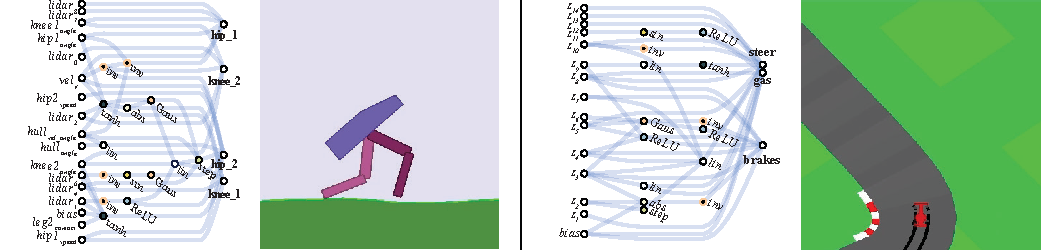
\includegraphics[width=1\textwidth]{img/cover.pdf}       
\vskip -0.05in % useful knobs to optimize layout
    \caption      
    {     
        \textit{Examples of Weight Agnostic Neural Networks: Bipedal Walker (left), Car Racing (right)}
        \newline
		We search for architectures by deemphasizing weights. In place of training, networks are assigned a single shared weight value at each rollout. Architectures that are optimized for expected performance over a wide range of weight values are still able to perform various tasks without weight training.
    }         
    \label{fig:cover_diagram} 
\vskip -0.05in % useful knobs to optimize layout
\end{figure}

Decades of neural network research have provided building blocks with strong inductive biases for various task domains. Convolutional networks~\cite{lecun1995convolutional,fukushima1982neocognitron} are especially suited for image processing~\cite{cohen2016inductive}. Recent work~\cite{he2016powerful,ulyanov2018deep} demonstrated that even randomly-initialized CNNs can be used effectively for image processing tasks such as superresolution, inpainting and style transfer. Schmidhuber et al.~\cite{evolino} have shown that a randomly-initialized LSTM~\cite{lstm} with a learned linear output layer can predict time series where traditional reservoir-based RNNs~\cite{jaeger2004harnessing,reservoir} fail. More recent developments in self-attention~\cite{vaswani2017attention} and capsule~\cite{sabour2017dynamic} networks expand the toolkit of building blocks for creating architectures with strong inductive biases for various tasks. Fascinated by the intrinsic capabilities of randomly-initialized CNNs and LSTMs, we aim to search for \textit{weight agnostic neural networks}, architectures with strong inductive biases that can already perform various tasks with random weights.

% contributions
In order to find neural network architectures with strong inductive biases, we propose to search for architectures by deemphasizing the importance of weights. This is accomplished by \textbf{(1)} assigning a single shared weight parameter to every network connection and \textbf{(2)} evaluating the network on a wide range of this single weight parameter. In place of optimizing weights of a fixed network, we optimize instead for architectures that perform well over a wide range of weights. We demonstrate our approach can produce networks that can be expected to perform various continuous control tasks with a random weight parameter. As a proof of concept, we also apply our search method on a supervised learning domain, and find it can discover networks that, even without explicit weight training, can achieve a much higher than chance test accuracy of $\sim$ 92\% on MNIST.
%
We hope our demonstration of such weight agnostic neural networks will encourage further research exploring novel neural network building blocks that not only possess useful inductive biases, but can also learn using algorithms that are not necessarily limited to gradient-based methods.\footnote{We released a software toolkit not only to facilitate reproduction, but also to further research in this direction. Refer to the Supplementary Materials for more information about the code repository.
}
